%! Author = Wiktor Rostkowski, Mateusz Budzisz
%! Date = 29/04/2024

\chapter{Podsumowanie}
\label{ch:podsumowanie}

\section{Napotkane wyzwania}
\label{sec:napotkane-wyzwania}

Największym wyzwaniem, z jakim zespół projektowy musiał się zmierzyć, był częściowy rozpad grupy, w wyniku którego zespół zmniejszył się o połowę.
To znaczące uszczuplenie liczby członków wpłynęło na zdolność zespołu do realizacji wszystkich zaplanowanych funkcjonalności.
W rezultacie projekt nie był w stanie w pełni zrealizować integracji z komunikacją miejską w Gdańsku, co było jedną z głównych funkcji przewidzianych w początkowym planie.
Ograniczenia te zmusiły zespół do priorytetyzacji innych elementów projektu oraz do poszukiwania alternatywnych rozwiązań, aby sprostać ograniczeniom zasobów i czasu.

Drugim największym wyzwaniem była implementacja kalendarza, który umożliwia planowanie zwiedzania w wybrane dni za pomocą funkcji przeciągnij i upuść.
Kalendarz ten uwzględnia godziny otwarcia atrakcji turystycznych oraz proponowany czas zwiedzania każdej atrakcji.
Algorytm kalendarza musi pilnować wszystkich tych ograniczeń, aby zaplanowany harmonogram był możliwy do zrealizowania w rzeczywistości.
Dodatkowo, możliwość zmiany czasu przeznaczonego na zwiedzanie przez użytkownika wprowadziła kolejny poziom skomplikowania, wymagając dynamicznej aktualizacji planu.
Ta funkcjonalność musiała również uwzględniać różne scenariusze i wyjątkowe przypadki, takie jak zmiany godzin otwarcia atrakcji w dni świąteczne czy nieprzewidziane zamknięcia, co dodatkowo komplikowało implementację.

\begin{figure}[H]
    \centering
    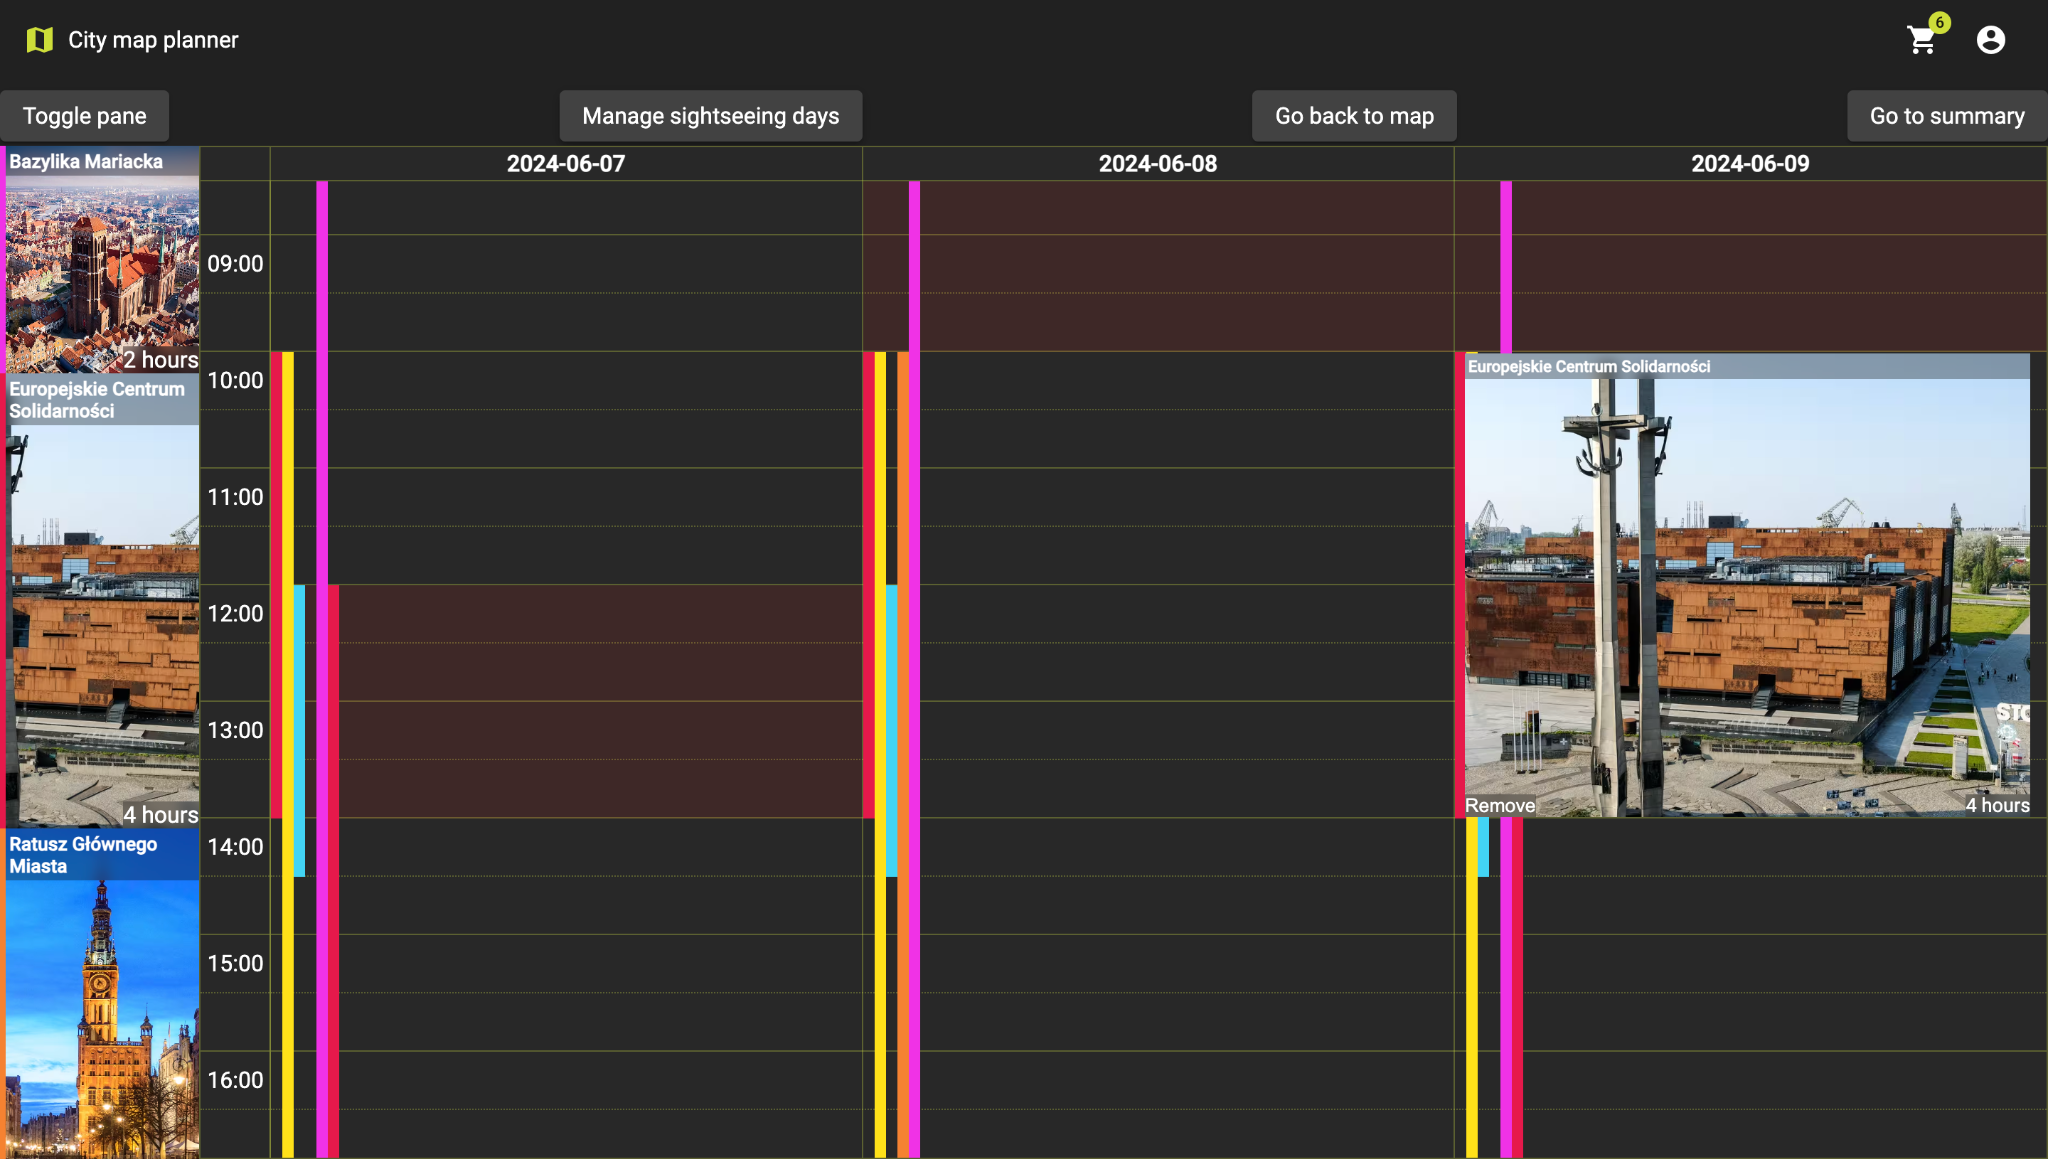
\includegraphics[width=1\textwidth]{attachments/t1}
    \caption{Screenshot przykładowego użycia kalendarza}
\end{figure}

Trzecim wyzwaniem, przed którym stanął zespół projektowy, była integracja menedżera punktów zainteresowania (POI) ze sztuczną inteligencją.
System co godzinę zapisuje snapshot stron internetowych atrakcji i porównuje je z wcześniejszymi wersjami w celu wykrycia zmian.
W przypadku wykrycia zmian, dane są przesyłane do modelu GPT-4 od OpenAI w celu ekstrakcji godzin otwarcia, co częściowo automatyzuje proces aktualizacji informacji.
Sztuczna inteligencja zwraca dane w formacie tabelki markdown z wartościami wymagającymi normalizacji.
Przetwarzanie tych zdenormalizowanych danych przed zapisaniem ich do finalnej tabeli w bazie danych stanowiło znaczące wyzwanie.
Ponadto konieczne było uwzględnienie i pokrycie wielu przypadków anomalii generowanych przez AI, co dodatkowo skomplikowało ten proces.
Wyzwanie to wymagało nie tylko solidnej wiedzy technicznej, ale także elastyczności w dostosowywaniu systemu do różnych formatów i źródeł danych.

\begin{figure}[H]
    \centering
    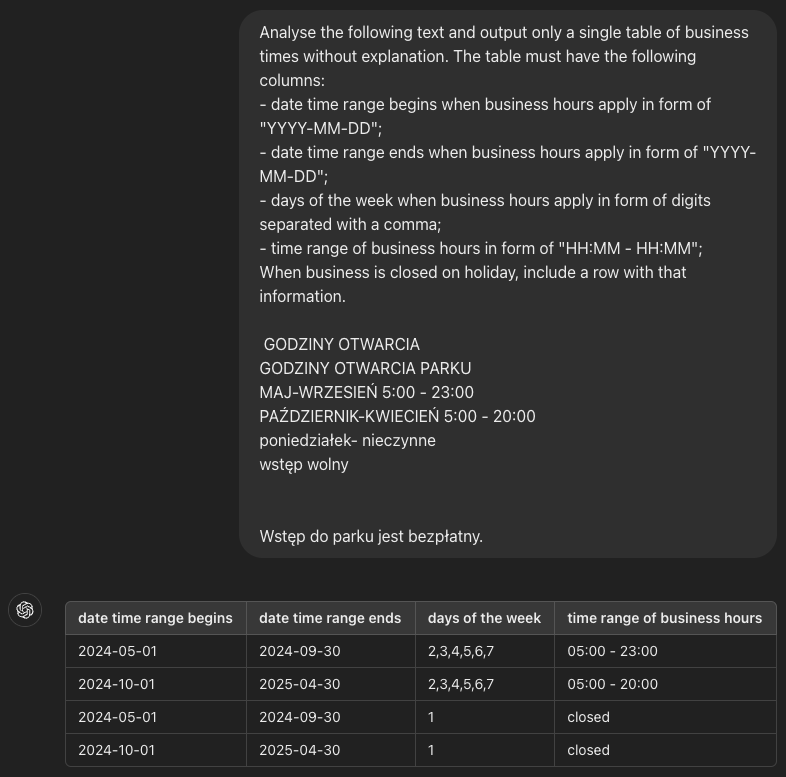
\includegraphics[width=1\textwidth]{attachments/t2}
    \caption{Przykład analizy AI}
\end{figure}

\section{Łączny nakład pracy}
\label{sec:laczny-naklad-pracy}

Łączny czas poświęcony przez członków zespołu na realizację tego projektu wyniósł 363 godziny.
Ten czas obejmował szeroki zakres działań, w tym analizę wymagań, projektowanie architektury systemu, implementację poszczególnych modułów, testowanie funkcjonalności oraz naprawianie błędów.
W ramach tych godzin zespół przeprowadzał także spotkania planistyczne i statusowe, konsultacje z interesariuszami, a także sesje programowania ekstremalnego, aby zapewnić, że wszystkie elementy projektu są zgodne z założeniami i spełniają oczekiwania użytkowników końcowych.

\section{Indywidualne wkłady pracy}
\label{sec:indywidualne-wklady-pracy}

\subsection{Mateusz Budzisz}
\label{subsec:mateusz-budzisz}

Bezpośrednio na projekt przeznaczyłem 253 godziny.
Jestem autorem pomysłu pracy dyplomowej oraz kierownikiem projektu.
Do moich obowiązków należało: organizacja cotygodniowych spotkań, przygotowanie infrastruktury docelowej, stworzenie i utrzymywanie repozytorium oraz ogólnie pojęta organizacja całości projektu.

W znacznej większości zaimplementowałem zarówno backend, jak i frontend systemu, co stanowiło kluczowy element techniczny projektu.
Dodatkowo, większość rozdziałów pracy dyplomowej jest mojego autorstwa, co odzwierciedla moje zaangażowanie i wkład merytoryczny w dokumentację projektu.

Pomimo moich wszelkich starań, aby wspierać innych członków zespołu, w tym poprzez propozycje wspólnych sesji programowania oraz udostępnienie prywatnych materiałów szkoleniowych, nie udało mi się przekonać ich do systematycznej pracy na rzecz projektu.
Starałem się aktywnie motywować i wspierać zespół, jednak spotkałem się z brakiem odpowiedniego zaangażowania z ich strony.
Moje wysiłki w zakresie organizacji i koordynacji prac projektowych, jak również znaczny wkład w rozwój techniczny i dokumentacyjny projektu, były kluczowe dla jego postępu i finalizacji.

\subsection{Wiktor Rostkowski}
\label{subsec:wiktor-rostkowski}

TODO

\section{Wnioski}\label{sec:wnioski}
Prace nad projektem rozpoczęły się pod koniec 2023 roku, w momencie sformowania zespołu projektowego podczas VI semestru studiów.
Zespół miał na celu ukończenie projektu do 18 czerwca 2024 roku, co wynikało z terminu narzuconego przez uczelnię oraz przyjętego bufora bezpieczeństwa.

Początkowo zespół planował realizację wszystkich zaplanowanych funkcjonalności, opierając się na komercyjnym doświadczeniu większości jego członków.
Niestety, projekt został tylko częściowo zrealizowany zgodnie z założeniami.
Główne trudności pojawiły się w momencie, gdy zespół stracił połowę swoich członków, co spowodowało, że zakres projektu stał się zbyt obszerny do ukończenia przez pozostałych członków.

Pomimo tych trudności, projekt zachował spójność graficzną, a jego kod cechuje się wysoką jakością i zgodnością ze standardami aplikacji biznesowych.
Zespół zdołał zrealizować minimalny wartościowy produkt, który przejawia duży potencjał na dalszy rozwój, szczególnie jeśli Urząd Miasta Gdańsk byłby zainteresowany jego wdrożeniem.

Wybrana technologia do realizacji projektu nie sprawiała problemów, co pozwoliło na sprawne przeprowadzenie prac.
Metodologia RAD (Rapid Application Development) okazała się doskonale dopasowana do charakteru projektu, a wyrafinowane potoki ciągłej integracji aplikacji znacząco przyczyniły się do ukończenia projektu w terminie oraz równoległego rozdzielania pracy pomiędzy członków zespołu.

W trakcie realizacji projektu, zespół projektowy zdobył wiele cennych doświadczeń i umiejętności, które z pewnością będą miały pozytywny wpływ na ich przyszłe kariery zawodowe.

\chapter*{Załączniki}
\begin{itemize}
    \item Tekst pracy dyplomowej (na płycie CD)
    \item Kod źródłowy projektu (na płycie CD)
\end{itemize}
